\section{Diagramas de Casos de Uso}
	En esta sección se presentan los casos de uso diseñados con base en los RF, RNF y RN. Por razones de espacio, están separados por los módulos del sistema.
	
	\subsection{Módulo de Gestión de Usuarios}
	Los casos de uso de este módulo permitirán la creación y mantenimiento de cuentas de usuario, así como la asignación de seguridad en los accesos a la aplicación. 

	\begin{figure}[htbp!]
		\centering
			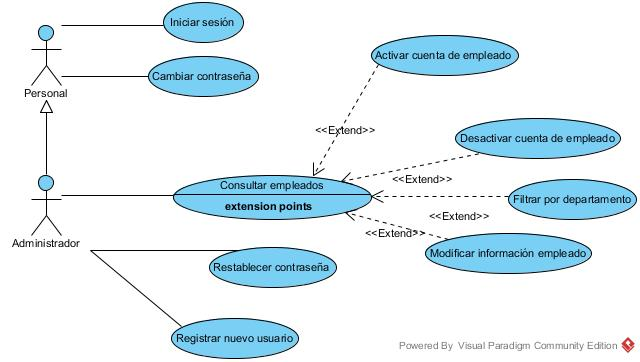
\includegraphics[width=0.8\textwidth]{images/Trabajo/cugestion}
		\caption{Diagrama de Casos de Uso. Módulo Gestión de Usuarios}
		\label{diagrama de cu}
	\end{figure}
	
	\subsection{Módulo Correspondencia Externa}
	Los casos de uso de este módulo permitirán registrar, turnar, responder, consultar, dar seguimiento, cancelar, atender, notificar y autorizar a los oficios que llegan al CMPL.
	
	\begin{figure}[htbp!]
		\centering
			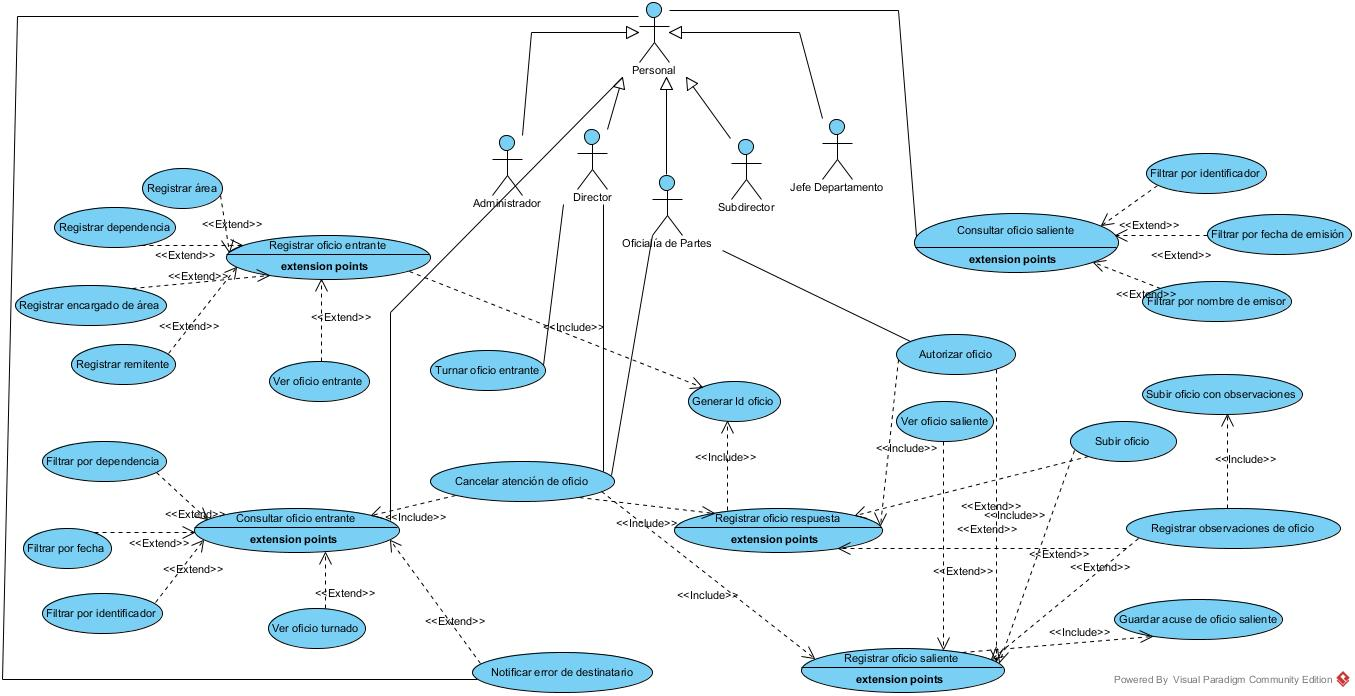
\includegraphics[width=0.8\textwidth]{images/Trabajo/CorrespondenciaExterna}
		\caption{Diagrama de Casos de Uso. Módulo Correspondencia Externa}
		\label{diagrama de cu}
	\end{figure}
	
	\subsection{Módulo Correspondencia Interna}
	Los casos de uso de este módulo permitirán la comunicación interna del CMPL, llevada mediante memorándums. 
	
	\begin{figure}[htbp!]
		\centering
			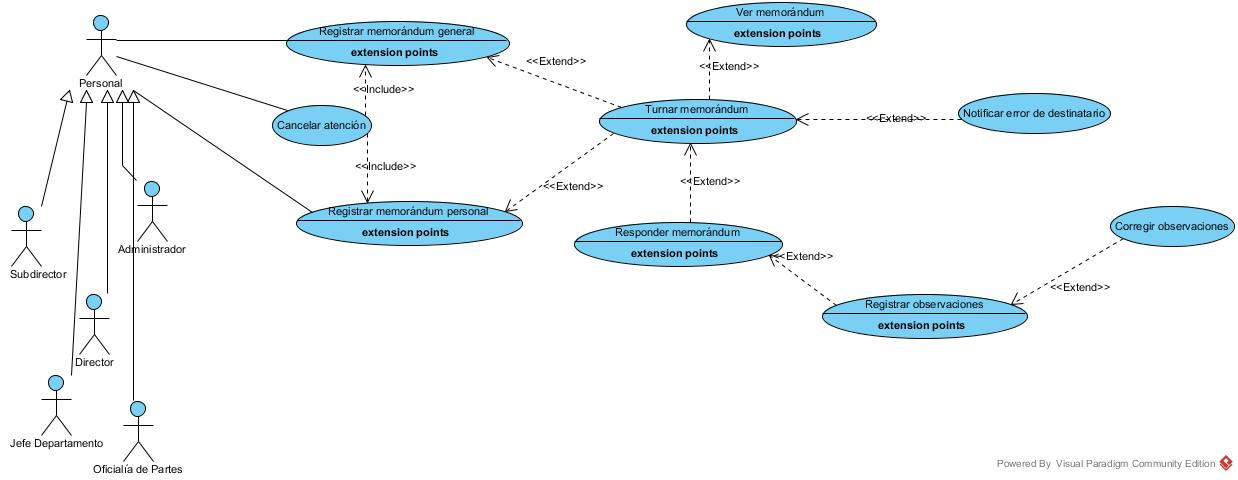
\includegraphics[width=0.8\textwidth]{images/Trabajo/CorrespondenciaInterna}
		\caption{Diagrama de Casos de Uso. Módulo Correspondencia Interna}
		\label{diagrama de cu}
	\end{figure}
%%%%%%%%%%%%%%%%%%%%%%%%%%%%%%%%%%%%% Casos de uso gestión de usu	
	\begin{UseCase}{CU1}{Iniciar Sesión}{Para poder utilizar la aplicación web es necesario que el usuario se autentique dentro de ella, ya que se necesita registrar la fecha de cuándo fue la última vez que inició sesión (para consultas administrativas), para que se le pueda desplegar la pantalla correspondiente y pueda ver su correspondencia personal, así como tener las configuraciones necesarias para reducir el tiempo de registro de oficios y memorándums.}
		\UCitem{Versión}{0.1}
		\UCitem{Actor}{Personal.}
		\UCitem{Propósito}{Que el personal del CMPL pueda hacer uso total de la aplicación}
		%\UCitem{Resumen}{Ayudar al personal del CMPL a tener un control de acceso a la aplicación.}
		\UCitem{Entradas}{Email, password.}
		\UCitem{Salidas}{Pantalla de bienvenida.}
		\UCitem{Precondiciones}{El personal debe estar registrado en la BD.}
		\UCitem{Postcondiciones}{El personal puede hacer uso de la aplicación.}
		\UCitem{Referencia}{-}
		\UCitem{Errores}{Error en la conexión a la base de datos. Si el personal ingresa mal su nombre de usuario y/o contraseña mostrará mensaje en pantalla 'Correo institucional y/o contraseña incorrectos, Intento de nuevo'.}
		\UCitem{Autor}{Ian Castañeda.}
		\UCitem{Revisó}{Oscar Alcántara.}
	\end{UseCase}

\begin{itemize}	
	\item Trayectoria principal:
		\begin{enumerate}
			\item El actor solicita iniciar sesión presionando el botón “Acceder” en la \IUref{IU1}.
			\item La aplicación solicita al actor que se identifique mostrando la pantalla \IUref{IU2}.
			\item El actor ingresa su correo institucional y contraseña en la interfaz.
			\item El actor solicita autenticación en la aplicación pulsando el botón “Iniciar sesión”. 
			\item La aplicación hace la consulta a la base de datos con los datos introducidos.
			\item La aplicación verifica que el usuario y la contraseña sean correctos.
			\item La aplicación verifica el tipo de usuario que se autenticó.
			\item Fin de caso de uso.

		\end{enumerate}
	\item Trayectorias alternativas:
		\begin{itemize}
			\item Trayectoria alternativa A: Si los datos introducidos no son correctos.
				\begin{enumerate}
					\item La aplicación muestra el mensaje \IUref{MSG1} pidiendo verificar correo institucional y/o contraseña.
					\item Continua en trayectoria principal en paso 3.
				\end{enumerate}
			\item Trayectoria alternativa B: Si es Director.
				\begin{enumerate}
					\item La aplicación muestra la pantalla \IUref{IU27}.
					\item Continua trayectoria principal.
				\end{enumerate}
			\item Trayectoria alternativa C: Si es Oficialía de partes.
				\begin{enumerate}
					\item La aplicación muestra la pantalla \IUref{IU3}.
					\item Continua trayectoria principal.
				\end{enumerate}
			\item Trayectoria alternativa D: Si es Jefe de Departamento o Subdirector.
				\begin{enumerate}
					\item La aplicación muestra la pantalla \IUref{IU26}.
					\item Continua trayectoria principal.
				\end{enumerate}
			\item Trayectoria alternativa E: Si es Administrativo.
				\begin{enumerate}
					\item La aplicación muestra la pantalla \IUref{IU28}.
					\item Continua trayectoria principal.
				\end{enumerate}
		\end{itemize}
\end{itemize}

\newpage
%%%%%%%%%%%%%%%%%%%%%%%%%%%%%%%%%%%%%%%%%%%%%%%%%%%%%%%%%%%%%%%%%%%%%
	\begin{UseCase}{CU2}{Registrar nuevo usuario}{Existen cambios en la administración del CMPL o llegan empleados nuevos, es necesario que los nuevos se registren en la aplicación web para que puedan hacer uso de ésta y así también se pueda mantener el directorio interno del CMPL actualizado.}
		\UCitem{Versión}{0.1}
		\UCitem{Actor}{Administrador.}
		\UCitem{Propósito}{Registrar a nuevos usuarios en la aplicación para que puedan hacer uso de ella.}
		%\UCitem{Resumen}{Ayudar al personal del CMPL a tener un control de acceso a la aplicación.}
		\UCitem{Entradas}{Nombre, ApPaterno, ApMaterno, Email, Extensión, URLCV, RolId, ÁreaId, CargoID}
		\UCitem{Salidas}{Mensaje Cuenta creada correctamente}
		\UCitem{Precondiciones}{Tener al menos un nuevo usuario para registrar.}
		\UCitem{Postcondiciones}{Usuario registrado en la BD.}
		%\UCitem{Referencia}{-}
		\UCitem{Errores}{Error en la conexión a la base de datos.Error en los datos introducidos}
		\UCitem{Autor}{Ian Castañeda.}
		\UCitem{Revisó}{Oscar Alcántara.}
	\end{UseCase}
	
			\begin{itemize}
				\item Trayectoria principal:
					\begin{enumerate}
						\item El actor da clic en el menú de herramientas administrativas.
						\item La aplicación muestra el menú de herramientas administrativas.
						\item El actor da clic en la opción ``Gestionar usuarios''.
						\item La aplicación muestra la pantalla \IUref{IU32}, de gestión de usuarios.
						\item El actor da clic en el botón ``Nuevo usuario''.
						\item La aplicación muestra la pantalla \IUref{33}, de registro de nuevos usuarios.
						\item El actor llena los campos con los datos requeridos por el formulario.
						\item El actor da clic en ``Registrar''.
						\item La aplicación verifica que el Nombre, Apellido Paterno, Apellido Materno y Correo Electrónico no sean parte de otro usuario registrado en la aplicación. \textsl{Trayectoria alternativa A}
						\item La aplicación verifica que la información ingresada en los dos campos de contraseña sean idénticos. \textsl{Trayectoria alternativa B}
						\item La aplicación registra los datos del nuevo usuario.
						\item La aplicación muestra la pantalla \IUref{IU32}, con un mensaje de confirmación que dice ``Cuenta de usuario creada correctamente''.
					\end{enumerate}
				\item Trayectorias alternativas:
					\begin{itemize}
						\item Trayectoria alternativa A: Cuando los datos ingresados en la aplicación ya han sido registrados anteriormente.
							\begin{enumerate}
								\item La aplicación muestra la pantalla \IUref{IU33}, con el mensaje de ``Ya hay un registro con los datos de este usuario''. Regresa al paso 7.
							\end{enumerate}
						\item Trayectoria alternativa B: Cuando las contraseñas ingresadas no coinciden.
							\begin{enumerate}
								\item La aplicación muestra la pantalla \IUref{IU33}, con el mensaje de ``Las contraseñas introducidas no coinciden''. Regresa al paso 7.
							\end{enumerate}
					\end{itemize}
			\end{itemize}

\newpage
%%%%%%%%%%%%%%%%%%%%%%%%%%%%%%%%%%%%%%%%%%%%%%%%%%%%%%%%%%%%%%%%%%%%%
\begin{UseCase}{CU3}{Modificar usuarios}{En ocasiones puede darse el caso de que un registro no tiene la información correcta de un empleado o de que esa información haya cambiado, por lo que es necesario que la aplicación web proporcione una forma de poder editar dichos datos y así mantener la información de los empleados actualizada.}
		\UCitem{Versión}{0.1}
		\UCitem{Actor}{Administrador.}
		\UCitem{Propósito}{Mantener actualizada los datos de los usuarios.}
		%\UCitem{Resumen}{Ayudar al personal del CMPL a tener un control de acceso a la aplicación.}
		\UCitem{Entradas}{Datos a cambiar. IdUsuario, Nombre, ApPaterno, ApMaterno, Email, Extensión, URLCV, RolId, CargoId, ÁreaId}
		\UCitem{Salidas}{Usuario actualizado correctamente}
		\UCitem{Precondiciones}{El personal debe estar registrado en la BD.}
		\UCitem{Postcondiciones}{Usuario actualizado}
		%\UCitem{Referencia}{-}
		\UCitem{Errores}{Error en la conexión a la base de datos. Error en datos introducidos}
		\UCitem{Autor}{Ian Castañeda.}
		\UCitem{Revisó}{Oscar Alcántara.}
	\end{UseCase}
			
			\begin{itemize}
				\item Trayectoria principal:
					\begin{enumerate}
						\item El actor da clic en el menú de herramientas administrativas.
						\item La aplicación muestra el menú de herramientas administrativas.
						\item El actor da clic en la opción ``Gestionar usuarios''.
						\item La aplicación muestra la pantalla \IUref{IU32}, de gestión de usuarios.
						\item El actor selecciona de la tabla que se muestra en \IUref{IU32} el usuario que desea editar.
						\item El actor selecciona la opción ``Modificar datos'' del menú de acciones del usuario a modificar.
						\item La aplicación muestra la pantalla \IUref{IU34}, de modificación de usuarios.
						\item El actor modifica los campos con los datos requeridos por el formulario.
						\item El actor da clic en ``Guardar''.
						\item La aplicación verifica que el Nombre, Apellido Paterno, Apellido Materno y Correo Electrónico no sean parte de otro usuario registrado en la aplicación. \textsl{Trayectoria alternativa A}
						\item La aplicación actualiza los datos del nuevo usuario.
						\item La aplicación muestra la pantalla \IUref{IU32}, con un mensaje de confirmación que dice ``Datos de usuario modificados correctamente''.
					\end{enumerate}
				\item Trayectorias alternativas:
					\begin{itemize}
						\item Trayectoria alternativa A: Cuando los datos ingresados en la aplicación ya han sido registrados anteriormente.
							\begin{enumerate}
								\item La aplicación muestra la pantalla \IUref{IU34}, con el mensaje de ``Ya hay un registro con los datos de este usuario''. Regresa al paso 7.
							\end{enumerate}
					\end{itemize}
			\end{itemize}
			
\newpage
%%%%%%%%%%%%%%%%%%%%%%%%%%%%%%%%%%%%%%%%%%%%%%%%%%%%%%%%%%%%%%%%%%%%%
\begin{UseCase}{CU4}{Desactivar cuenta de usuario}{Esto se dará cuando un empleado deje de laborar dentro del CMPL. Su cuenta no podrá ser eliminada de la aplicación web, ya que a esa cuenta seguramente habrá oficios y memorándums vinculados, pero sí se podrá deshabilitar para que el usuario de esa cuenta ya no pueda entrar a la aplicación web.	}
		\UCitem{Versión}{0.1}
		\UCitem{Actor}{Administrador.}
		\UCitem{Propósito}{Que el actor pueda desactivar la cuenta de un usuario.}
		%\UCitem{Resumen}{}
		\UCitem{Entradas}{Nombre del usuario, estatus}
		\UCitem{Salidas}{Mensaje Ususario desactivado correctamente.}
		\UCitem{Precondiciones}{Que el usuario tenga el estado de activado}
		\UCitem{Postcondiciones}{La aplicación ya no permitirá el acceso al usuario}
		\UCitem{Referencia}{CU}
		\UCitem{Errores}{Error en la conexión a la base de datos.}
		\UCitem{Autor}{Ian Castañeda.}
		\UCitem{Revisó}{Oscar Alcántara.}
	\end{UseCase}		

			\begin{itemize}
				\item Trayectoria principal:
					\begin{enumerate}
						\item El actor da clic en el menú de herramientas administrativas.
						\item La aplicación muestra el menú de herramientas administrativas.
						\item El actor da clic en la opción ``Gestionar usuarios''.
						\item La aplicación muestra la pantalla \IUref{IU32}, de gestión de usuarios.
						\item El actor selecciona de la tabla que se muestra en \IUref{IU32} el usuario que desea desactivar.
						\item El actor selecciona la opción ``Inhabilitar usuario'' del menú de acciones del usuario a modificar.
						\item La aplicación cambia el estado de ``Activo'' a ``Inactivo'' del usuario seleccionado en la base de datos.
						\item La aplicación muestra la pantalla \IUref{IU32}, con un mensaje de confirmación que dice ``Usuario inhabilitado correctamente''.
					\end{enumerate}
			\end{itemize}
			
\newpage
%%%%%%%%%%%%%%%%%%%%%%%%%%%%%%%%%%%%%%%%%%%%%%%%%%%%%%%%%%%%%%%%%%%%%
\begin{UseCase}{CU5}{Activar cuenta de usuario}{En el caso de que un exempleado regrese a trabajar al CMPL y haya tenido cuenta en la aplicación web anteriormente, en la aplicación se podrá volver a habilitar su cuenta para que siga trabajando. Sus oficios y memorándums anteriores estarán ahí.}
		\UCitem{Versión}{0.1}
		\UCitem{Actor}{Administrador.}
		\UCitem{Propósito}{Que el actor pueda activar la cuenta del usuario que regrese a laborar en el centro.}
		%\UCitem{Resumen}{Ayudar al personal del CMPL a tener un control de acceso a la aplicación.}
		\UCitem{Entradas}{Nombre, estado.}
		\UCitem{Salidas}{Mensaje 'Usuario activado correctamente.'}
		\UCitem{Precondiciones}{El usuario a activar debe estar desactivado.}
		\UCitem{Postcondiciones}{El usuario puede acceder a la aplicación.}
		%\UCitem{Referencia}{-}
		\UCitem{Errores}{Error en la conexión a la base de datos.}
		\UCitem{Autor}{Ian Castañeda.}
		\UCitem{Revisó}{Oscar Alcántara.}
	\end{UseCase}
	
			\begin{itemize}
				\item Trayectoria principal:
					\begin{enumerate}
						\item El actor da clic en el menú de herramientas administrativas.
						\item La aplicación muestra el menú de herramientas administrativas.
						\item El actor da clic en la opción ``Gestionar usuarios''.
						\item La aplicación muestra la pantalla \IUref{IU32}, de gestión de usuarios.
						\item El actor selecciona de la tabla que se muestra en \IUref{IU32} el usuario que desea activar.
						\item El actor selecciona la opción ``Habilitar usuario'' del menú de acciones del usuario a modificar.
						\item La aplicación cambia el estado de ``Inactivo'' a ``Activo'' del usuario seleccionado en la base de datos.
						\item La aplicación muestra la pantalla \IUref{IU32}, con un mensaje de confirmación que dice ``Usuario habilitado correctamente''.
					\end{enumerate}
			\end{itemize}
			
\newpage
%%%%%%%%%%%%%%%%%%%%%%%%%%%%%%%%%%%%%%%%%%%%%%%%%%%%%%%%%%%%%%%%%%%%%
\begin{UseCase}{CU6}{Filtrar usuarios por departamento}{En el caso de que se desee consultar el directorio interno del CMPL por departamento se podrá hacer. Bastará con elegir el departamento deseado y pedirle a la aplicación web que regrese únicamente los datos de los usuarios de ese departamento.}
		\UCitem{Versión}{0.1}
		\UCitem{Actor}{Administrador.}
		\UCitem{Propósito}{Encontrar a un usuario registrado de una manera más rápida.}
		%\UCitem{Resumen}{}
		\UCitem{Entradas}{Nombre del departamento.}
		\UCitem{Salidas}{Usuarios cargados a ese departamento.}
		\UCitem{Precondiciones}{Que el departamento este registrado, que los usuarios esten registrados y cargados a un departamento.}
		\UCitem{Postcondiciones}{Actualización de la base de datos.}
		%\UCitem{Referencia}{-}
		\UCitem{Errores}{Error en la conexión a la base de datos.}
		\UCitem{Autor}{Ian Castañeda.}
		\UCitem{Revisó}{Oscar Alcántara.}
	\end{UseCase}
			
			\begin{itemize}
				\item Trayectoria principal:
					\begin{enumerate}
						\item El actor va a la sección de menú y selecciona ``Directorio CMPL''.
						\item La aplicación muestra la pantalla \IUref{IU35}, con una tabla que muestra por departamento el directorio interno del CMPL por nombre completo, cargo, extensión y correo electrónico.
						\item El actor selecciona el departamento que desea consultar en específico en la opción ``Buscar por departamento''.
						\item El actor da clic en el botón ``Consultar''.
						\item La aplicación muestra la pantalla \IUref{IU35}, con la información del personal del departamento seleccionado. 
					\end{enumerate}
			\end{itemize}
			
\newpage
%%%%%%%%%%%%%%%%%%%%%%%%%%%%%%%%%%%%%%%%%%%%%%%%%%%%%%%%%%%%%%%%%%%%%%%%%%

\begin{UseCase}{CU7}{Restablecer contraseña de usuario}{En ocasiones a los usuarios se les olvida su contraseña de acceso a la aplicación web. Cuando eso ocurra podrán acudir con el administrador de la aplicación a pedir que les asigne una nueva contraseña que ellos deberán modificar posteriormente. El administrador podrá restablecer las contraseñas de los usuarios desde la aplicación.}
		\UCitem{Versión}{0.1}
		\UCitem{Actor}{Administrador.}
		\UCitem{Propósito}{Permitir recuperar el acceso al personal que lo requiera}
		%\UCitem{Resumen}{Ayudar al personal del CMPL a tener un control de acceso a la aplicación.}
		\UCitem{Entradas}{Contraseña nueva.}
		\UCitem{Salidas}{Contraseña actualizada.}
		\UCitem{Precondiciones}{Que el usuario no pueda acceder a la aplicación.}
		\UCitem{Postcondiciones}{Actualización de la contraseña en la BD.}
		%\UCitem{Referencia}{-}
		\UCitem{Errores}{Error en la conexión a la base de datos.}
		\UCitem{Autor}{Ian Castañeda.}
		\UCitem{Revisó}{Oscar Alcántara.}
	\end{UseCase}
			
			\begin{itemize}
				\item Trayectoria principal:
					\begin{enumerate}
						\item El actor da clic en el menú de herramientas administrativas.
						\item La aplicación muestra el menú de herramientas administrativas.
						\item El actor da clic en la opción ``Gestionar usuarios''.
						\item La aplicación muestra la pantalla \IUref{IU32}, de gestión de usuarios.
						\item El actor elije el usuario que desea editar y da clic al botón ``Acciones'' del menú de opciones de ese usuario.
						\item La aplicación muestra el menú de opciones del usuario seleccionado.
						\item El actor da clic en ``Restablecer contraseña''.
						\item La aplicación muestra la pantalla \IUref{IU36}, de restablecimiento de contraseña.
						\item El actor teclea una nueva contraseña.
						\item El actor vuelve a teclear la nueva contraseña.
						\item El actor da clic al botón ``Cambiar contraseña''.
						\item La aplicación verifica que ambos campos de contraseña coincidan. \textsl{Trayectoria alternativa A}
						\item La aplicación verifica que la contraseña no sea menor a 6 dígitos. \textsl{Trayectoria alternativa B}
						\item La aplicación cambia la contraseña del usuario seleccionado.
						\item La aplicación muestra la pantalla \IUref{IU32}, de gestión de usuarios, con el mensaje ``Contraseña de usuario modificada correctamente''.

					\end{enumerate}
				\item Trayectorias alternativas:
					\begin{itemize}
						\item Trayectoria alternativa A:
							\begin{enumerate}
								\item La aplicación muestra un mensaje de error.
							\end{enumerate}
					\end{itemize}
			\end{itemize}
			
			\newpage
			
\begin{UseCase}{CU8}{Cambiar contraseña}{El usuario puede cambiar su contraseña directamente en la aplicación web en caso de que necesite cambiarla, ya sea porque se ha restablecido por parte del administrador o porque el usuario así lo desea.}
		\UCitem{Versión}{0.1}
		\UCitem{Actor}{Personal.}
		\UCitem{Propósito}{Que el personal del CMPL pueda cambiar su contraseña.}
		\UCitem{Resumen}{Ayudar al personal del CMPL a mantener la seguridad de su información.}
		\UCitem{Entradas}{Contraseña anterior, contraseña nueva.}
		\UCitem{Salidas}{Contraseña actualizada.}
		\UCitem{Precondiciones}{Haber iniciado sesión.}
		\UCitem{Postcondiciones}{Contraseña actualizada.}
		%\UCitem{Referencia}{-}
		\UCitem{Errores}{Error en la conexión a la base de datos.}
		\UCitem{Autor}{Ian Castañeda.}
		\UCitem{Revisó}{Oscar Alcántara.}
	\end{UseCase}
				
			\begin{itemize}
				\item Trayectoria principal:
					\begin{enumerate}
						\item El actor va a la sección de correspondencia 
						\item El actor da clic en el menú ``Mi perfil''.
						\item La aplicación muestra el menú del perfil de usuario.
						\item El actor da clic en la opción ``Configuración''.
						\item La aplicación muestra la pantalla \IUref{IU37}, de Mi perfil.
						\item El actor selecciona el botón ``Cambiar contraseña''.
						\item La aplicación muestra la pantalla \IUref{IU36}, de restablecimiento de contraseña.
						\item El actor teclea una nueva contraseña.
						\item El actor vuelve a teclear la nueva contraseña.
						\item El actor da clic al botón ``Cambiar contraseña''.
						\item La aplicación verifica que ambos campos de contraseña coincidan. \textsl{Trayectoria alternativa A}
						\item La aplicación verifica que la contraseña no sea menor a 6 dígitos. \textsl{Trayectoria alternativa B}
						\item La aplicación cambia la contraseña del usuario seleccionado.
						\item La aplicación muestra la pantalla \IUref{IU37}, de Mi perfil, con el mensaje ``Contraseña modificada correctamente''.
					\end{enumerate}
				\item Trayectorias alternativas:
					\begin{itemize}
						\item Trayectoria alternativa A:
							\begin{enumerate}
								\item La aplicación muestra un mensaje de error.
							\end{enumerate}
					\end{itemize}
			\end{itemize}

\newpage

